\documentclass[a4paper,12pt]{article}

\usepackage{mystyle}
\usepackage{gensymb}


\usepackage{scalerel}
\usepackage{stackengine}

\graphicspath{ {images/} }


% https://tex.stackexchange.com/questions/5461/is-it-possible-to-change-the-size-of-an-arrowhead-in-tikz-pgf
\usetikzlibrary{arrows.meta}


\DeclareMathOperator{\Image}{Im}

\definecolor{pink}{RGB}{218, 3, 174}
\definecolor{violet}{RGB}{148, 0, 211}
\definecolor{green}{RGB}{0, 153, 0}
\definecolor{orange}{RGB}{255, 153, 0}
\definecolor{blue}{RGB}{5, 73, 255}


% https://tex.stackexchange.com/a/101138/135045

\newcommand\widesim[1]{\ThisStyle{%
  \setbox0=\hbox{$\SavedStyle#1$}%
  \stackengine{-.1\LMpt}{$\SavedStyle#1$}{%
    \stretchto{\scaleto{\SavedStyle\mkern.2mu\sim}{.5150\wd0}}{.6\ht0}%
  }{O}{c}{F}{T}{S}%
}}

\newcommand{\BigMiddleThree}{\;\left|\vphantom{\begin{pmatrix} 0\\0\\0 \end{pmatrix}}\right.\;}
\newcommand{\BigMiddleFour}{\;\left|\vphantom{\begin{pmatrix} 0\\0\\0\\0 \end{pmatrix}}\right.\;}


% https://tex.stackexchange.com/questions/63531/how-to-write-quotation-marks-in-math-environment
\DeclareMathSymbol{\mlq}{\mathord}{operators}{``}
\DeclareMathSymbol{\mrq}{\mathord}{operators}{`'}


\DeclareMathOperator{\Imag}{Im}


% https://tex.stackexchange.com/questions/544453/undefined-control-sequence-after-paragraph
\renewcommand{\paragraph}[1]{\noindent\textbf{#1}\quad}


% https://tex.stackexchange.com/questions/36851/skipping-line-after-proof-in-proof-environment#comment73553_36851
\newcommand{\proofindent}{\hspace*{\fill}\par\vspace{0.5em}\noindent}



\author{Алексеев Василий}


\title{Семинар 8}
\date{31 марта + 4 апреля 2023}


\begin{document}
  \maketitle
  
  \tableofcontents

  \thispagestyle{empty}
  
  \newpage
  
  \pagenumbering{arabic}


  \section{Inv (Diag 1. Part 2)}
  
  \subsection{Инвариантность характеристического многочлена}
  
  Пусть $\phi\colon X \hm\to X$ линейное преобразование вещественного линейного пространства $X$ размерности~$n$.
  Пусть в~$X$ выбран некоторый базис $e \hm= (\bds e_1, \ldots, \bds e_n)$, в котором матрица преобразования~$\phi$ есть $A \hm\in \RR^{n \times n}$.
  Тогда собственные значения \emph{преобразования} (то есть все числа $\lambda \hm\in \RR$, такие что $\phi(\bds x) \hm= \lambda \bds x$ для хотя бы одного ненулевого вектора $\bds x$) можно было искать как действительные корни характеристического уравнения \emph{матрицы} этого преобразования:
  \begin{equation}\label{eq:characteristic}
    \det (A - \lambda E) = 0
  \end{equation}
  
  В этом месте стоило задаться вопросом: а корректен ли такой способ поиска собственных значений?
  В том смысле, не получится ли так, что у характеристического уравнения для матрицы~$A$ преобразования~$\phi$ в базисе~$e$ будут одни корни, а у характеристического уравнения для матрицы~$A'$ \emph{того же} преобразования~$\phi$, но уже в \emph{другом} базисе~$e'$, корни будут другие?  % TODO: comma needed not needed?..
  Пусть ``старый'' и ``новый'' базисы связаны матрицей перехода: $e' \hm= e S$, $S \hm\in \RR^{n\times n}$, $\det S \hm{\not=} 0$.
  Тогда матрица~$A'$ в ``новом'' базисе~$e'$ так выражается через матрицу~$A$ в ``старом'' базисе~$e$: $A' \hm= S^{-1} A S$.
  Распишем характеристический многочлен матрицы~$A'$:
  \begin{equation*}
  \begin{split}
    \det(A' - \lambda E)
      &= \det(S^{-1} A S - \lambda S^{-1} S)\\
      &= \det\bigl(S^{-1} \cdot (A - \lambda E) \cdot S\bigr)\\
      &= \det S^{-1} \cdot \det(A - \lambda E) \cdot \det S
      = \det(A - \lambda E)
  \end{split}
  \end{equation*}
  
  То есть характеристические многочлены матриц одного и того же преобразования в разных базисах совпадают!
  Получается, будут одинаковыми все коэффициенты в характеристических многочленах, стоящие при $\lambda$ в одинаковых степенях:
  \begin{equation*}
    (-1)^n \lambda^n + (-1)^{n-1} \lambda^{n-1} \Sp A' + \ldots + \det A'
      = (-1)^n \lambda^n + (-1)^{n-1} \lambda^{n-1} \Sp A + \ldots + \det A
  \end{equation*}
  То есть у матриц $A$ и $A'$ преобразования $\phi$ совпадают след и определитель.
  Эти величины являются \emph{инвариантами}, связанными с преобразованием, то есть они не зависят от выбора базиса.
  А раз совпадают характеристические многочлены, то и корни характеристических уравнений матриц $A$ и $A'$ будут одинаковыми (вплоть до кратностей).
  Поэтому характеристическое уравнение \emph{матрицы}~(\ref{eq:characteristic}) можно называть характеристическим уравнением \emph{преобразования}.
  
  
  \subsection{Собственные подпространства преобразования}
  
  Пусть найдено собственное значение $\lambda \hm\in \RR$ преобразования.
  Рассмотрим множество всех векторов~$L_{\lambda}$, каждый из которых под действием $\phi$ остаётся параллелен себе с коэффициентом~$\lambda$:
  \begin{equation}\label{eq:proper-subspace}
    L_{\lambda} = \{\bds x \in X \mid \phi(\bds x) = \lambda \bds x\}
  \end{equation}
  то есть $L_{\lambda}$ состоит из собственных векторов, относящихся к собственному значению~$\lambda$, а также из нулевого вектора (который по определению собственным вектором не является).
  Покажем, что \emph{$L_{\lambda}$ есть подпространство в $X$}.
  Пусть $\bds x_1, \bds x_2 \hm\in L_{\lambda}$.
  Тогда для их суммы имеем:
  \[
    \phi(\bds x_1 + \bds x_2) = \phi(\bds x_1) + \phi(\bds x_2) = \lambda \bds x_1 + \lambda \bds x_2 = \lambda (\bds x_1 + \bds x_2)
  \]
  то есть сумма $\bds x_1 \hm+ \bds x_2$ тоже вектор из~$L_{\lambda}$.
  Аналогично $\alpha \bds x \hm\in L_{\lambda}$, $\alpha \hm\in \RR$, $\bds x \hm\in L_{\lambda}$.
  Получается, $L_{\lambda}$ замкнуто относительно операций сложения векторов и умножения вектора на число, поэтому является подпространством~$X$.
  
  Подпространство~$L_{\lambda}$ называется \emph{собственным подпространством, соответствующим собственному значению $\lambda$}.
  Собственные векторы, относящиеся к $\lambda$, являются ненулевыми векторами~$L_{\lambda}$.
  
  Раз $\lambda$ собственное значение, то оно будет корнем характеристического уравнения преобразования~(\ref{eq:characteristic})\footnote{Почему это верно? То есть обычно как, находим корни, и они~---~собственные значения. Почему верно наоборот: что если собственное значение, то обязательно корень?}.
  Пусть кратность $\lambda$ как корня есть $p \hm\geq 1$.
  Что можно сказать о \emph{размерности собственного подпространства $L_{\lambda}$, соответствующего $\lambda$}?
  Очевидно, $\dim L_{\lambda} \hm\geq 1$.
  Также очевидно, что $\dim L_{\lambda} \hm\leq n \hm= \dim X$.
  Можно ли указать более точную верхнюю границу для $\dim L_{\lambda}$?
  Допустим, $\dim L_{\lambda} \hm\equiv d \hm> p$.
  Тогда в подпространстве $L_{\lambda}$ можно выбрать $d$ линейно независимых векторов.
  Дополним эту систему векторов до базиса $e'$ пространства~$X$.
  Что можно сказать про матрицу~$A'$ преобразования~$\phi$ в этом базисе?
  Так как первые $d$ векторов базиса $e'$ собственные, то:
  \[
    A' = \left(\vphantom{\begin{matrix} 1 \\ 1 \\ 1 \\ 1 \\ 1 \\ 1 \\ 1 \end{matrix}}\right.
      \underbrace{
        \begin{matrix}
          \lambda   & 0         & 0         & \ldots & 0\\
          0         & \lambda   & 0         & \ldots & 0\\
          0         & 0         & \lambda   & \ldots & 0\\
          \vdots    & \vdots    & \vdots    & \ddots & \vdots\\
          0         & 0         & 0         & \ldots & \lambda\\
          \vdots    & \vdots    & \vdots    & \ddots & \vdots\\
          0         & 0         & 0         & 0      & 0\\
        \end{matrix}
      }_{d}
      \ \ \ \underbrace{  % TODO: kostylevatiy space between matrices here
        \begin{matrix}
          \cdot  & \cdot  & \ldots & \cdot\\
          \cdot  & \cdot  & \ldots & \cdot\\
          \cdot  & \cdot  & \ldots & \cdot\\
          \vdots & \vdots & \ddots & \vdots\\
          \cdot  & \cdot  & \ldots & \cdot\\
          \vdots & \vdots & \ddots & \vdots\\
          \cdot  & \cdot  & \ldots & \cdot\\
        \end{matrix}
      }_{n - d}
    \left.\vphantom{\begin{matrix} 1 \\ 1 \\ 1 \\ 1 \\ 1 \\ 1 \\ 1 \end{matrix}}\right)
  \]
  
  Но характеристическое уравнение такой матрицы\footnote{Из-за небольшой коллизии обозначений в этом месте пришлось вместо ``стандартного'' $\det(A \hm- \lambda E) \hm= 0$ написать $\det(A \hm- l E) \hm= 0$, то есть \emph{переменная в уравнении} есть $l$, потому что $\lambda$ уже означает \emph{некоторое собственное значение}.}:
  \[
    \det(A' - l E) = (\lambda - l)^d \cdot (\ldots) = 0
  \]
  и у него $\lambda$, очевидно, корень кратности как минимум $d$.
  Но такого не может быть, потому что корни вплоть до кратностей инварианты, а изначальная кратность $p$ по предположению меньше $d$.
  Поэтому верно следующее утверждение.
  
  \begin{proposition}
    Пусть $\lambda$ есть корень характеристического уравнения преобразования $\phi$~(\ref{eq:characteristic}) кратности $p \hm\geq 1$.
    Тогда размерность соответствующего собственного подпространства $L_{\lambda}$ не превосходит~$p$.
  \end{proposition}
  
  
  \subsection{Инвариантные подпространства преобразования}
  
  Посмотрим ещё раз на собственное подпространство $L_{\lambda}$~(\ref{eq:proper-subspace}).
  Заметим, что если $\bds x \hm\in L_{\lambda}$, то
  \[
    \phi\bigl(\phi(\bds x)\bigr) = \phi(\lambda \bds x) = \lambda \phi(\bds x)
  \]
  то есть образ $\phi(\bds x)$ любого вектора $\bds x$ из $L_{\lambda}$ также лежит в~$L_{\lambda}$.
  Тогда про подпространство~$L_{\lambda}$ говорят, что оно является инвариантным относительно преобразования~$\phi$.
  
  \begin{definition}
    Подпространство $L'$ линейного пространства $L$ называется \emph{инвариантным} относительно преобразования $\phi\colon L \hm\to L$, если $\forall \bds x \hm\in L' \hm\to \phi(\bds x) \hm\in L'$.  % TODO: phi: X->X or L->L (consistency?)
    Иными словами, если $\phi(L') \subseteq L'$.
  \end{definition}
  
  Пусть вектор $\bds x_1$ собственный, соответствующий~$\lambda$, то есть $\phi(\bds x_1) \hm= \lambda \bds x_1$ и $\bds x_1$ ненулевой.
  Тогда множество векторов $L_{\bds x_1} \hm= \{\bds x \hm\in X \hm\mid \bds x \hm= \alpha \bds x_1, \alpha \hm\in \RR\}$, очевидно, будет одномерным подпространством.
  Но оно также будет инвариантно относительно~$\phi$:
  \[
    \phi(\alpha \bds x_1) \hm= \alpha \phi(\bds x_1) = \underbrace{\alpha \cdot \lambda}_{\beta \in \RR} \bds x_1 = \beta \bds x_1
  \]
  (то есть образ любого вектора вида $\alpha \bds x_1$ также лежит в $L_{\bds x_1}$, более того, $\alpha \bds x_1$ будет собственным при $\alpha \hm{\not=} 0$, так как $\phi(\alpha \bds x_1) \hm= \alpha \cdot \lambda \bds x_1 \hm= \lambda \cdot \alpha \bds x_1$).
  Итого, на каждый собственный вектор~$\bds x_1$ преобразования натянуто одномерное инвариантное подпространство.
  
  % We do not want to copy lecture notes...
  %Но верно и обратное.
  %Пусть вектор $\bds x_1$ ненулевой и является базисом в одномерном инвариантном подпространстве~$L_{\bds x_1}$.
  %Покажем, что тогда $\bds x_1$ обязательно собственный:
  %\[
    %\bds x_1 \in L_{\bds x_1}, \phi(L_{\bds x_1}) \subseteq L_{\lambda}
    %\Rightarrow \phi(\bds x_1) \in L_{\bds x_1}
    %\Rightarrow \phi(\bds x_1) = \lambda \bds x_1,\ \lambda \in \RR
  %\]
  %
  %Сформулируем кратко в виде утверждения наблюдение, описанное выше.
  %
  %\begin{proposition}
    %Собственные векторы преобразования~$\phi$ и только они являются базисными векторами одномерных подпространств, инвариантных относительно~$\phi$.
  %\end{proposition}
  
  Ести ли какие-нибудь ``другие'' примеры инвариантных подпространств?
  
  \begin{example}
    Для любого преобразования $\phi\colon X \hm\to X$ инвариантными будут нулевое подпространство $\{\bds 0\}$ и всё пространство~$X$.
  \end{example}
  
  \begin{example}
    Если $\lambda_1$ и $\lambda_2$ есть два различных собственных значения преобразования $\phi$, то инвариантной будет сумма соответствующих собственных подпространств: $L_{\lambda_1} \hm+ L_{\lambda_2}$.
  \end{example}
  
  \begin{example}
    Вспомним про номер, в котором рассматривается преобразование~$\phi$ геометрического трёхмерного пространства векторов~$\mathcal L$, суть которого~---~ортогональная проекция на прямую $\mathcal L_1\colon x \hm= y \hm= z$ (базис ортонормированный).
    Формула преобразования:
    $
      \phi(\bds x) \hm= \frac{(\bds x, \bds a)}{|\bds a^2|} \bds a
    $,
    где $\bds a$ есть направляющий вектор прямой~$\mathcal L_1$.
    Матрица преобразования: $A \hm= \frac{1}{3} \left(\begin{smallmatrix}
      1 & 1 & 1\\
      1 & 1 & 1\\
      1 & 1 & 1
    \end{smallmatrix}\right)$.
    Какие подпространства будут инвариантны относительно~$\phi$?
    
    Очевидно, нулевое подпространство $\{\bds 0\}$ и всё пространство $\mathcal L$ инвариантны.
    
    Найдутся ли \emph{одномерные} инвариантные подпространства?
    Да~---~очевидно, это сама сама прямая~$\mathcal L_1$~(\ref{fig:inv-subspaces}).
    А также любая прямая, перпендикулярная~$\mathcal L_1$.
    Например, прямая с направляющим вектором $\bds b = (2, -1, -1)^T$.
    
    Найдутся ли \emph{двумерные} инвариантные подпространства?
    Да~---~очевидно, это плоскость, перпендикулярная $\mathcal L_1$.
    А также... любая плоскость, \emph{содержащая} $\mathcal L_1$~(\ref{fig:inv-subspaces}).
    То есть все плоскости вида $\{t_1 \bds a \hm+ t_2 \bds b \hm\mid t_1, t_2 \hm\in \RR\}$, где $\bds b$ есть некоторый вектор, не параллельный~$\bds a$.
    
    \begin{figure}[h]
      \centering
  
      \includegraphics[width=0.75\columnwidth]{inv-subspaces}
  
      \caption{Подпространства трёхмерного геометрического векторного пространства: одномерное и двумерные~---~инвариантные относительно преобразования~$\phi$ ортогонального проектирования на прямую~$\mathcal L_1$. (Плоскости и прямые нарисованы как геометрические объекты, с ``видимой'' и ``невидимой'' частью, но это сделано лишь для лучшего восприятия рисунка~---~на самом деле под прямыми и плоскостями в данном случае имеются в виду векторные подпространства, для которых понятие ``относительного расположения'' не такое, как для их ``геометрических аналогов''.)}
      \label{fig:inv-subspaces}
    \end{figure}
    
    Заметим, что
    $
      \phi(\bds a) \hm= 1 \cdot \bds a
    $,
    то есть вектор $\bds a$ собственный, соответствующий собственному значению $\lambda \hm= 1$.
    И через него, как через собственный вектор, проходит одномерное инвариантное подпространство.
    Так и получилось: это подпространство и есть прямая~$\mathcal L_1$.
    Также получается, что
    $
      \phi(\bds b) \hm= \bds 0 \hm= 0 \cdot \bds b
    $,
    то есть вектор $\bds b$ тоже собственный, но соответствующий собственному значению $\lambda \hm= 0$.
  \end{example}
  
  
  \section{Задачи}
  
  
  \subsection{\# 24.42(1)}
  
  Найти собственные значения и собственные векторы дифференцирования $D\colon \mathcal P^{(n)} \hm\to \mathcal P^{(n)}$ как линейного преобразования пространства многочленов степени не выше $n$.
  
  \begin{solution}
    \hfill\par
    \emph{Способ 1: ``Из определения''}.
    
    Ищем собственный многочлен в виде:
    \begin{equation}\label{eq:p24-42-p-t}
      p(t) = a_0 + a_1 t + a_2 t^2 + \ldots + a_{n - 1} t^{n - 1} + a_n t^n
    \end{equation}
    
    Его образ:
    \[
      \bigl(D(p)\bigr)(t) = a_1 + 2 a_2 t + \ldots + n a_n t^{n - 1}
    \]
    
    Раз $p(t)$ собственный, то должно найтись число $\lambda \hm\in \RR$ (собственное значение):
    \begin{equation}
    \begin{split}
      D(p) = \lambda p
        \leftrightarrow a_1 &+ 2 a_2 t + \ldots + n a_n t^{n - 1}\\
                      = \lambda a_0 &+ \lambda a_1 t + \ldots + \lambda a_{n - 1} t^{n - 1} + \lambda a_n t^n
    \end{split}
    \end{equation}
    
    Приравнивая коэффициенты при $t$ в одинаковых степенях у многочленов ``слева'' и ``справа'', получаем систему:
    \[
      \left\{
        \begin{aligned}
          &a_1 = \lambda a_0\\
          &2 a_2 = \lambda a_1\\
          &\vdots\\
          &n a_n = \lambda a_{n - 1}\\
          &0 = \lambda a_n
        \end{aligned}
      \right.
    \]
    
    Из последнего уравнения следует две возможности: $\lambda \hm{\not=} 0$ (и $a_n$ обязательно ноль) и $\lambda \hm= 0$ (тогда $a_n$ любой).
    Если $\lambda \hm{\not=} 0$, то из предпоследнего уравнения следует $a_{n - 1} \hm= 0$.
    И далее, все коэффициенты получаются нулевыми, вплоть до $a_1$ (второе уравнение системы) и $a_0$ (первое уравнение).
    То есть в рассматриваемом случае $p \hm\equiv 0$.
    Но собственный по определению не нулевой.
    Поэтому выбор $\lambda \hm{\not=} 0$ ни к чему не привёл.
    
    Пусть теперь $\lambda \hm= 0$.
    Из предпоследнего уравнения следует $a_n \hm= 0$.
    И таким образом зануляются все коэффициенты вплоть до $a_2$ (второе уравнение системы) и $a_1$ (первое уравнение).
    Но... про $a_0$ так ничего и не известно!
    То есть $a_0$ может быть любым.
    Получается, любой многочлен вида $p(t) \hm= a_0$, $a_0 \hm{\not=} 0$ будет собственным для $\lambda \hm= 0$.
    И если бы требовалось, например, найти максимальную по числу линейно независимую систему из собственных векторов преобразования~$D$, то это была бы, например, система из одного вектора $\{-17.5\}$.
    
    
    \emph{Способ 2: ``Стандартная схема''}.
    
    Введём базис в пространстве многочленов $\mathcal P^{(n)}$.
    Например:
    \[
      e = (1, t, t^2, \ldots, t^{n - 1}, t^n)
    \]
    
    В этом базисе у многочлена $p$~(\ref{eq:p24-42-p-t}) будет координатный столбец $\xi \hm= (a_0, a_1, \ldots, a_{n - 1}, a_n)^T$, а у его образа $D(p)$ будет столбец $\eta \hm= (a_1, 2 a_2, \ldots, n a_n, 0)$.
    
    В базисе $e$ у преобразования $D$ будет матрица $A \hm\in \RR^{(n + 1) \times (n + 1)}$:
    \[
      A \xi = \eta
      \quad\leftrightarrow\quad A \begin{pmatrix}
        a_0\\
        a_1\\
        \vdots\\
        a_{n - 1}\\
        a_n
      \end{pmatrix} = \begin{pmatrix}
        a_1\\
        2 a_2\\
        \vdots\\
        n a_n\\
        0
      \end{pmatrix}
      \quad\Rightarrow\quad A = \begin{pmatrix}
        0      & 1      & 0      & \ldots & 0      & 0\\
        0      & 0      & 2      & \ldots & 0      & 0\\
        \vdots & \vdots & \vdots & \ddots & \vdots & \vdots\\
        0      & 0      & 0      & \ldots & 0      & n\\
        0      & 0      & 0      & \ldots & 0      & 0
      \end{pmatrix}
    \]
    
    Характеристическое уравнение матрицы:
    \[
      \det(A - \lambda E) = 0
    \]
    \[
      \begin{vmatrix}
        -\lambda & 1        & 0      & \ldots & 0        & 0\\
        0        & -\lambda & 2      & \ldots & 0        & 0\\
        \vdots   & \vdots   & \vdots & \ddots & \vdots   & \vdots\\
        0        & 0        & 0      & \ldots & -\lambda & n\\
        0        & 0        & 0      & \ldots & 0        & -\lambda
      \end{vmatrix} = 0
      \Rightarrow \lambda = 0\quad \mbox{(кратность $n + 1$)}
    \]
    
    Собственные векторы для единственного найденного $\lambda \hm= 0$:
    \[
      (A - \lambda E) \xi = 0
    \]
    \[
      \begin{pmatrix}
        0      & 1      & 0      & \ldots & 0      & 0\\
        0      & 0      & 2      & \ldots & 0      & 0\\
        \vdots & \vdots & \vdots & \ddots & \vdots & \vdots\\
        0      & 0      & 0      & \ldots & 0      & n\\
        0      & 0      & 0      & \ldots & 0      & 0
      \end{pmatrix} \begin{pmatrix}
        a_0\\
        a_1\\
        \vdots\\
        a_{n - 1}\\
        a_n
      \end{pmatrix} = 0
      \Rightarrow \left\{
        \begin{aligned}
          &a_0 \in \RR\\
          &a_1, a_2, \ldots, a_n = 0
        \end{aligned}
      \right.
    \]
    
    То есть собственные векторы, соответствующие $\lambda \hm= 0$, это константные ненулевые многочлены.
    Собственное подпространство, соответствующее $\lambda \hm= 0$, это одномерное подпространство с базисом, например, $\{-17.5\}$.
  \end{solution}
  
  
  \subsection{\# 24.70}
  
  Пусть $\phi\colon L \hm\to L$ линейное преобразование линейного пространства $X$.
  Доказать, что любое подпространство $L' \hm\subseteq L$, содержащее $\Imag\phi$, инвариантно.
  
  \begin{solution}
    Проверим инвариантность подпространства~$L'$ просто по определению:
    \[
      \bds x \hm\in L' \Rightarrow \phi(\bds x) \in \Imag\phi \subseteq L'
    \]
    
    То есть, да, инвариантно.
    
    (Решение получилось до неприличия коротким, поэтому попробуем далее немного ``раскрутить сюжет'' и заметить ``что-нибудь интересное''.)
    
    Так как $\Imag\phi \hm\subseteq L' \hm\subseteq L$, то
    \[
      \dim\Imag\phi \hm\leq \dim L' \hm\leq \dim L
    \]
    
    Минимальное по размерности подпространство $L'$, удовлетворяющее условию задачи, это $\Imag\phi$.
    Максимальное по размерности~---~это всё $L$.
    
    Если $L' \hm{\not=} L$, то существует ненулевое прямое дополнение $L''$ подпространства $L'$:
    \[
      L' \oplus L'' = L
    \]
    
    Выберем теперь базисы в $L'$ и $L''$.
    Пусть это будут базисы $p = (\bds p_1, \ldots, \bds p_k)$ и $q \hm= (\bds q_1, \ldots, \bds q_l)$ соответственно ($k \hm= \dim L'$, $l \hm= \dim L''$, $k \hm+ l \hm= \dim L \hm\equiv n$).
    Тогда можно в качестве базиса в~$L$ взять объединение базисов $p$ и $q$:
    \[
      e = (\bds p_1, \ldots, \bds p_k, \bds q_1, \ldots, \bds q_l)
    \]
    
    Какой будет матрица~$A$ преобразования~$\phi$ в этом базисе?
    Можно выписать её по столбцам.
    Так, первый столбец~---~это координаты $\phi(\bds p_1)$ в $e$.
    Единственное, что можно сказать про $\phi(\bds p_1)$~---~это то, что $\phi(\bds p_1) \hm\in \Imag\phi$, а потому и $\phi(\bds p_1) \hm\in L'$, и, значит, раскладывается по базису $p$.
    Аналогично и с образами остальных векторов базиса~$e$.
    Поэтому матрица~$A$ имеет вид:
    \[
      A = \begin{pmatrix}
        a_{11} & a_{12} & \ldots & a_{1n}\\
        a_{21} & a_{22} & \ldots & a_{2n}\\
        \vdots & \vdots & \ddots & \vdots\\
        a_{k1} & a_{k2} & \ldots & a_{kn}\\
        0      & 0      & 0      & 0\\
        0      & 0      & 0      & 0\\
        \vdots & \vdots & \ddots & \vdots\\
        0      & 0      & 0      & 0
      \end{pmatrix}
    \]
    
    Причём $\Rg A \hm= \dim\Imag\phi$, а потому из $k$ ненулевых строк можно максимум выбрать $\dim\Imag\phi$ линейно независимых.
    
    \medskip
    
    Пусть в качестве $L'$ выбрано просто $\Imag\phi$ (один из ``граничных случаев'', минимальное по размерности $L'$).
    Тогда в матрице преобразования первые $\Imag\phi$ строчек будут и ненулевыми, и линейно независимыми.
    Также можно заметить, что в этом случае размерность прямого дополнения~$L''$ получается равной:
    \[
      \dim L'' = \dim L - \dim L' = \dim L - \dim\Imag\phi = \dim\Ker\phi
    \]
    то есть равна размерности ядра преобразования $\Ker\phi$!
    Однако значит ли это, что $L''$ обязательно и есть ядро?..
    На самом деле, нет, может, и не ядро.
    Потому что если $\Ker\phi \hm\cap \Imag\phi \hm{\not=} \{\bds 0\}$, то их сумма не прямая и $\Ker\phi$ не будет прямым дополнением $\Imag\phi$\footnote{А у какого преобразования, например, ядро будет иметь ненулевое пересечение со множеством значений?}.
  \end{solution}
  
  
  \subsection{\# 24.55(1)}
  
  Пусть $\phi\colon \RR^{2\times 2} \hm\to \RR^{2\times 2}$ есть линейное преобразование квадратных матриц второго порядка, заданное формулой:
  \[
    \phi(X) = AX,\quad A = \begin{pmatrix}
      -4 & 0\\
      1 & 4
    \end{pmatrix}
  \]
  
  Надо найти собственные значения и максимальную линейно независимую систему собственных векторов преобразования~$\phi$.
  В случае, если эта система из собственных векторов может быть выбрана в качестве базиса, записать в нём матрицу преобразования~$\phi$.
  
  % TODO: not quite a good way to change stuff (in the middle of the process)...
  % https://tex.stackexchange.com/questions/256944/a-question-on-how-to-change-the-qed-symbol-of-amsthm
  \renewcommand\qedsymbol{$\blacksquare$}
  
  \begin{solution}
    Пойдём по ``стандартной схеме'': найдём собственные значения из характеристического уравнения $\det(A \hm- \lambda E) \hm= 0$, потом для каждого собственного значения~$\lambda_i$ будем искать собственные векторы как решения соответствующей однородной системы с матрицей $(A \hm- \lambda_i E)$.
    
    Характеристическое уравнение:
    \[
      \det(A - \lambda E) = 0
    \]
    \[
      \begin{vmatrix}
        -4 - \lambda & 0\\
        1 & 4 - \lambda
      \end{vmatrix} = 0 \Rightarrow \left\{
        \begin{aligned}
          &\lambda_1 = 4\\
          &\lambda_2 = -4
        \end{aligned}
      \right.
    \]
    
    Собственные векторы для~$\lambda_1$:
    \[
      (A - \lambda_1 E) \bds x = 0
    \]
    \[
      \begin{pmatrix}
        -8 & 0\\
        1 & 0
      \end{pmatrix} \begin{pmatrix}
        x_1\\
        x_2
      \end{pmatrix} = \begin{pmatrix}
        0\\
        0
      \end{pmatrix}
      \Rightarrow \boxed{
        \bds x_1 = \begin{pmatrix}
          0\\
          2023
        \end{pmatrix}
      }
    \]
    
    Собственные векторы можно либо просто подобрать, глядя на матрицу (и понимая при этом, сколько линейно независимых векторов должно получиться: в данном случае это всего один вектор $\bds x_1$, так как в системе $(A \hm- \lambda_1 E) \bds x \hm= \bds 0$ одна параметрическая неизвестная~---~переменная $x_2$).
    Либо можно просто по-честному решить систему, получив базис в пространстве решений (фундаментальную матрицу)~---~этот базис и будет давать максимальную линейно независимую систему собственных векторов для $\lambda_1$ (базис в соответствующем собственном подпространстве).
    
    Собственные векторы для~$\lambda_2$:
    \[
      (A - \lambda_2 E) \bds x = 0
    \]
    \[
      \begin{pmatrix}
        0 & 0\\
        1 & 8
      \end{pmatrix} \begin{pmatrix}
        x_1\\
        x_2
      \end{pmatrix} = \begin{pmatrix}
        0\\
        0
      \end{pmatrix}
      \Rightarrow \boxed{
        \bds x_2 = \begin{pmatrix}
          -8\\
          1
        \end{pmatrix}
      }
    \]
    
    Снова всего один собственный вектор, который тоже несложно подобрать из по сути единственного уравнения системы $x_1 \hm+ 8 x_2 \hm= 0$.
    
    Получается, нашли собственные векторы $\bds x_1$ и $\bds x_2$, их два.
    Можно взять в качестве базиса систему $e' \hm= \{\bds x_1, \bds x_2\}$.
    В этом базисе из собственных векторов матрица~$A'$ преобразования будет иметь вид:
    \[
      A' = \begin{pmatrix}
        4 & 0\\
        0 & -4
      \end{pmatrix}
    \]
    где на диагонали стоят собственные значения, которые соответствуют векторам базиса $e'$ из собственных векторов, так как $\phi(\bds x_1) \hm= \lambda_1 \bds x_1$ и $\phi(\bds x_2) \hm= \lambda_2 \bds x_2$.
    
    Нашли базис из собственных векторов, получили диагональный вид матрицы преобразования $\phi$.
    Преобразования квадратных матриц второго порядка $\RR^{2\times 2}$...
    размерности \emph{четыре}...
    Но мы нашли базис $\{\bds x_1, \bds x_2\}$~---~в котором всего \emph{два} вектора!?..
    
    \bigskip
    
    Какой сейчас год?..
    Какой сейчас год?..
    АААААААААААА!
  \end{solution}
\end{document}
